\documentclass[fleqn,10pt]{wlscirep}
\usepackage[utf8]{inputenc}
\usepackage[T1]{fontenc}
\usepackage{graphicx}
\usepackage{hyperref}
\usepackage{breakcites}
\usepackage{float}
\usepackage{textcomp}
\usepackage{amsmath}
\usepackage{textgreek}
\usepackage{authblk}
\usepackage{rotating}
\usepackage{booktabs}
\usepackage{longtable}
\usepackage{pdflscape}
\usepackage{lineno}
\usepackage{xcolor}
% \usepackage[
% style=numeric,
% citestyle=numeric-comp,
% backend=biber,
% doi=true,
% natbib=true,
% sorting=none
% ]{biblatex}
\usepackage{scalerel,xparse}

% To be able to use emojis
\NewDocumentCommand\emojismile{}{
 \scalerel*{
 
\includegraphics{smiling-face-with-smiling-eyes_1f60a.png}
 }{X}
}

%https://www.overleaf.com/project/5f918edd1afc380001feca0d
\title{Fine-scale Data Reveals Neighborhood Inequalities In Effects of Heat on Expressed Mood}

\author[1,*]{Matthew Cooper}
\author[2]{Jeremiah Osborne-Gowey}
\author[3]{Zheng Liu}
\author[4]{Portia Adade Williams}
\author[5]{Jie Liu}
\author[6]{Aaron Schwartz}
\author[7]{Patrick Baylis} 

\affil[1]{T.H. Chan School of Public Health, Harvard University}
\affil[2]{Environmental Studies Program, University of Colorado Boulder}
\affil[3]{Department of Geographical Sciences, University of Maryland College Park}
\affil[4]{University of Cape Town}
\affil[5]{School of Business, East China University of Science and Technology}
\affil[6]{University of Colorado Boulder}
\affil[7]{University of British Columbia}
\affil[*]{Corresponding Author: mcooper@hsph.harvard.edu}



\begin{abstract}
%Limit 150 words: https://www.nature.com/nclimate/about/content
%Actually there are lots of examples of articles with > 150 words, but I think we should keep it concise
Higher temperatures associated with climate change are expected to have major impacts on human mental health. Indeed, previous work has found strong associations between heat and mental health outcomes. These studies typically use data reported at the city or county level, and, to date, have found no difference in vulnerability based on income or race at coarse spatial scales. However, using expressed mood in a quarter of a billion geolocated tweets as a proxy for mental health status, we show that there are stark differences in the effects of heat depending on neighborhood characteristics. We find that increased temperatures worsen expressed mood in all areas, but that this effect is much stronger in poor and Black neighborhoods. We also find that the effect of heat on expressed mood is greatest in the early morning, supporting the hypothesis that heat affects mental health through a sleep quality pathway. This paper presents the first evidence of heterogeneity in the vulnerability of mental health to heat.
\end{abstract}
\begin{document}

\raggedbottom
\maketitle
\thispagestyle{empty}

\section*{Main}
%Overview
Climate change is impacting many aspects of human well-being. A large body of research has explored the ongoing impacts of climate change on agricultural outcomes, economic growth, and physical health \cite{pachauri2014climate}. However, academic and medical researchers have highlighted the relative paucity of empirical studies on the impacts of climate change on mental health \cite{Berry2018Apr, hayes_climate_2018}. While mental health is under-studied, it accounts for up 13\% of the global burden of disease, representing a major share of total human suffering \cite{Collins2011Jul}, leading to calls for more research into potential linkages between climate change and mental health \cite{Berry2018Apr, Collins2011Jul}. Researchers have begun to answer these calls, finding associations between climate disasters and post-traumatic stress \cite{Waite2017Dec, Raker2019Dec}, deteriorating environmental conditions and a sense of "ecological grief" \cite{Cunsolo2018Apr}, and linkages between higher temperatures and a variety of mental health outcomes \cite{baylis_weather_2018, Mullins2019Dec, Li2020Mar, Obradovich2018Oct}. Nevertheless, with average global temperatures projected to increase by 1.5\textdegree C within a decade \cite{allen2019technical}, more research is needed into the impacts of increased heat on mental health \cite{Berry2018Apr}, especially for identifying the most vulnerable communities.

%Theoretical: frameworks and pathways
Researchers have proposed a number of frameworks that focus on pathways by which temperature can affect mental health \cite{Berry2018Apr, Palinkas2020Apr, BerryETAL2010}. Work on biological mechanisms emphasizes the mental health effects from dehydration and other consequences of maintaining stable body temperature in high heat \cite{Lohmus2018Jul, sadiq_impact_2019}. Additionally, recent studies find nighttime temperatures affect sleep quality, with consequences for mental health \cite{Obradovich2017May, Mullins2019Dec}. Other studies point to linkages between increased temperatures, overall physical health and increases in injuries which can in turn affect mental health \cite{Berry2007, WHO2007}. Finally, exposure to higher temperatures can affect productivity and income \cite{kjellstrom_impact_2016, Burke2015Nov}, leading to second-order impacts on mental health outcomes \cite{Katz1997, CohnETAL2004, BouchamaETAL2007}.

%Empirical: Heat and mental health
Results from an emerging literature are beginning to demonstrate that higher temperatures can lead to deteriorating mental health. Multiple studies find strong evidence that higher temperatures are associated with increases in suicides in the United States \cite{Burke2018Aug, Mullins2019Dec, Dixon2007May} with other studies finding a similar relationship in locations around the world \cite{Qi2014Dec, Page2007Aug, Likhvar2011Jan}. Higher temperatures are also correlated with increased hospitalizations related to general mental health issues \cite{Obradovich2018Oct, Mullins2019Dec} and incidents related specific conditions like bipolar disorder and schizophrenia \cite{Lee2007Jan, Sung2013Feb}. Higher temperatures are also linked to increased mortality among people with pre-existing mental health disorders \cite{Hansen2008Oct}.

The effects of heat exposure on mental health are by now relatively well established, yet results from research conducted at national scales indicate surprisingly little heterogeneity in impacts, with consequences for our understanding of groups that are most vulnerable as well as potential adaptations to future heat stress. For example, a large study of temperature and suicide in the USA and Mexico found "no significant difference in suicide response to temperature between rich and poor municipalities or counties" \cite{Burke2018Aug}. Similarly, a national study found no effect of income as modifier of the effect of temperature on suicides, emergency department visits, or self-reported mental health status across the USA \cite{Mullins2019Dec}. A major challenge for these studies, however, is their reliance on data that is typically aggregated to the municipality or county level. As a consequence, these studies are often restricted to between-county metrics of vulnerability and cannot take into account neighborhood effects.

Findings from large-scale studies of relatively uniform vulnerability to heat are surprising given that minority groups and low-income people are more likely to be exposed to undesirable temperatures and less able to mitigate the effects of higher heat. For example, people from poorer socio-economic backgrounds are more likely to work outside rather than indoors \cite{Gubernot2014Oct}, more likely to rely on public transportation, bicycling, or walking instead of commuting in their own air-conditioned car \cite{Karner2015Dec}, and more likely to live in housing that is less insulated with poorer quality or no air-conditioning \cite{Samuelson2020Jun}. Many of these factors that expose low-income people to heat may be exacerbated and compounded for racial minorities. For example, Black Americans face discrimination in employment \cite{Reid2003, Kang2016, Penner2008} and housing access \cite{Desmond2015, Akbar2019}, forcing them into jobs and homes that may expose them to more heat. Additionally, policymakers have historically been less likely to take measures to address environmental hazards in Black neighborhoods \cite{Banzhaf2019}. Notably, there is often an intersectionality between different forms of vulnerability and oppression, with income and race likely having a compounding effect on vulnerability to environmental risks \cite{Kuran2020Nov}. Heterogeneity in vulnerability is also more pronounced within city regions rather than between cities, particularly in the United States where there can be considerable regional variability \cite{Cardona2012Jan}. Some studies find large differences in vulnerability between neighborhoods for a variety of impacts of heat on physical and mental health \cite{Belanger2015Mar, Uejio2011Mar}, as well as for vulnerability to other types of climate shocks like hurricanes \cite{ferre2019hurricane, Gruebner2015Jun}. Thus, there are strong reasons to expect heterogeneity in the impact of heat on mental health outcomes for different populations, particularly where socioeconomic, racial and other social inequities intersect, although there is little evidence of this to date. 

While public health data on mental health outcomes is not available at the neighborhood scale, spontaneous, in situ data from the social media platform Twitter can provide an important, inexpensive and timely proxy for mental health at extremely precise spatial and temporal scales. Many studies use the mood expressed in social media posts as an indicator of mental health \cite{Edo-Osagie2020Jul, Sinnenberg2016Dec}. For example, studies have used Twitter data to identify the onset of Post Traumatic Stress Disorder (PTSD) in individuals even before their formal diagnosis \cite{Reece2017Oct}. Similar methods applied to posts on Facebook can predict the onset of depression \cite{Eichstaedt2018Oct}. In London, day-to-day changes in mental health indicators derived from the text of tweets were associated with changes in mental health crisis episodes \cite{Kolliakou2020Feb}. Across the USA, more positive tweets are associated with a variety of metrics of human well-being \cite{Mitchell2013May}. Finally, the mood expressed in tweets has been strongly associated with local weather conditions \cite{baylis_weather_2018, hannak_tweetin_2012} and been used as evidence to support the temperature-suicide relationship \cite{Burke2018Aug}. Thus, posts on Twitter provide an proxy for mental health at fine enough spatial scales to examine neighborhood effects on vulnerability to higher temperatures. To explore how neighborhood conditions affect the relationship between heat and mental heath, we draw on a data set of 243 million geolocated tweets from across the continental United States covering the period 2009-2019, each paired with data on local weather and neighborhood conditions.

\section*{Results}

\subsection*{Overall Effect}
We examine the relationship between the mood expressed in tweets and the prevailing Wet Bulb Globe Temperature (WBGT), a temperature metric that accounts for dry-bulb temperature, humidity, wind speed, and solar radiation to more accurately describe the effects of heat on the human body \cite{budd2008wet}. We find higher temperatures are associated with worsened mood (Fig. \ref{fig:wbgt}) after controlling for a variety of fixed effects across all tweets. Mood is highest at 5\textdegree C WBGT (associated in our data set with a median dry bulb temperature on 12\textdegree C/54\textdegree F) with the largest declines between 20\textdegree -25\textdegree C WBGT (dry bulb 29\textdegree-36\textdegree C/84\textdegree-97\textdegree F). Mood also declines with colder temperatures (below 5\textdegree C WBGT), although only slightly. Dis-aggregating our analysis by metropolitan area and using alternative methods to estimate expressed mood all yield similar results (see Supplement).

\begin{figure}[H]
 \centering
 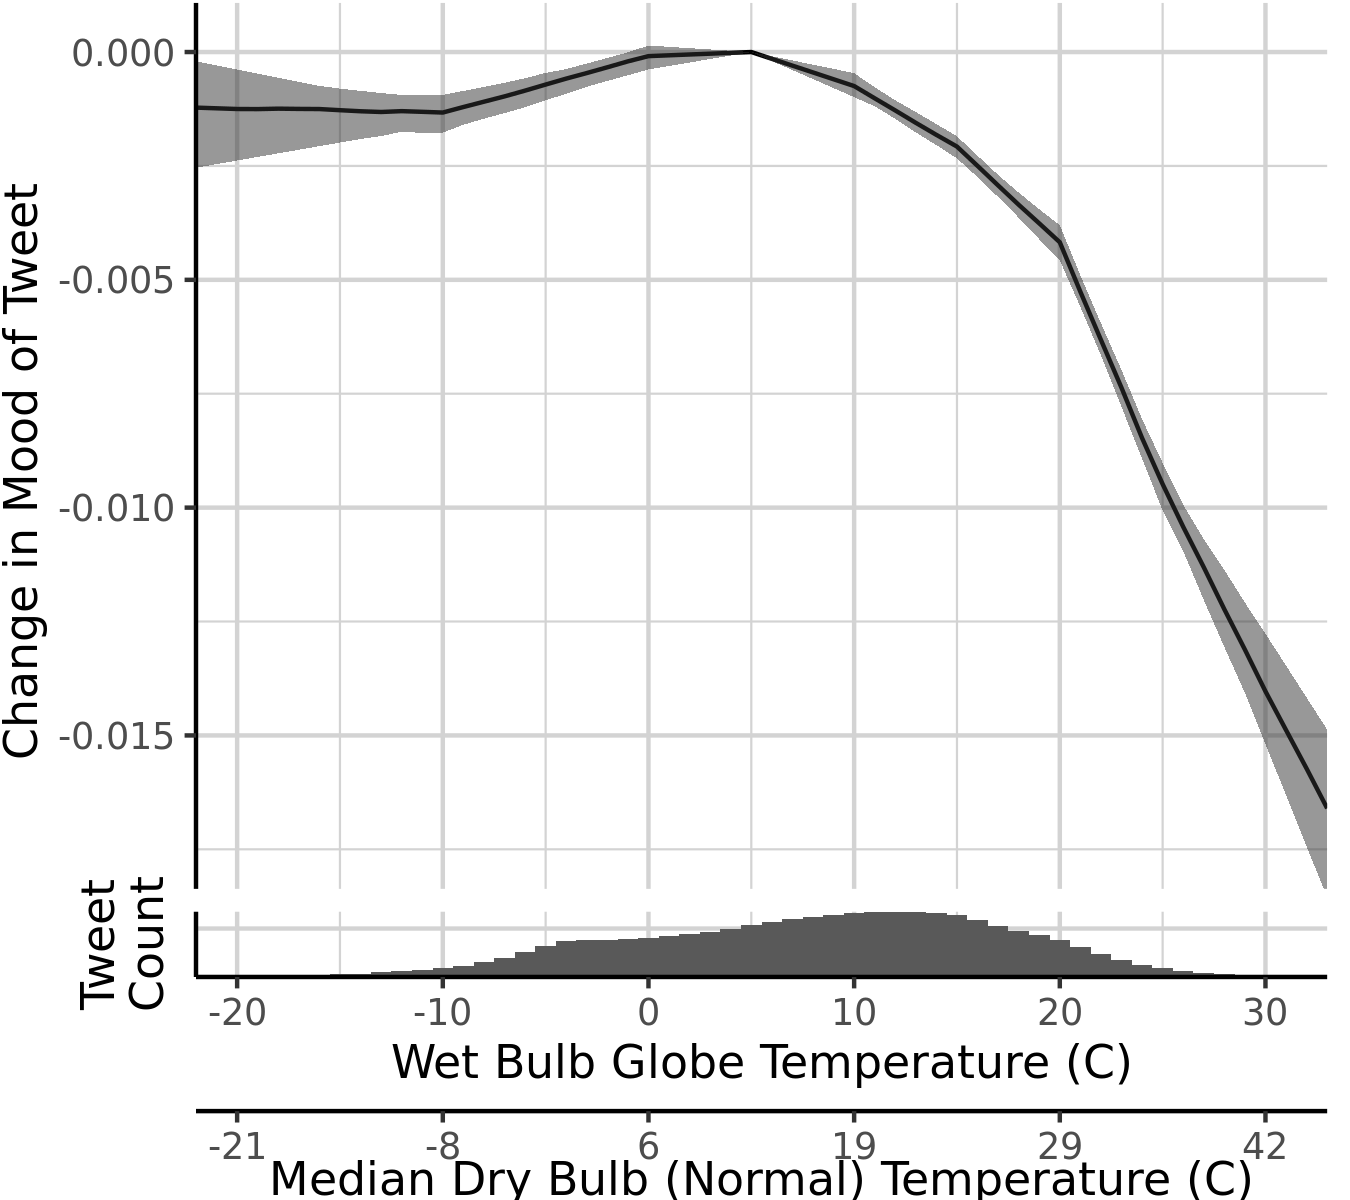
\includegraphics[width=0.5\linewidth]{../res/wbgt.png}
 \caption{Relationship between Wet Bulb Globe Temperature (WBGT) and expressed mood in tweets. As temperatures increase above 5\textdegree C WBGT, mood rapidly declines.}
 \label{fig:wbgt}
\end{figure}

We find that mean neighborhood income strongly moderates the relationship between temperature and mood (Fig. \ref{fig:hetero}), with large differences in mood between the poorest (5th percentile) and wealthiest (95th percentile) neighborhoods. As temperatures increase to a modest 20\textdegree C WBGT (29\textdegree C/84\textdegree F), mood increases in the wealthiest neighborhoods but decreases in the median and lowest income neighborhoods. The wealthiest neighborhoods do not see decreases in mood until temperatures exceed 20\textdegree C WBGT (29\textdegree C/84\textdegree F), at which point mood decreases relatively evenly regardless of neighborhood income percentile.

We also explored how neighborhood racial characteristics affect the relationship between temperature and mood, and we find the effects of heat are felt disproportionately in neighborhoods that are majority Black (Fig. \ref{fig:hetero}). Relative to an optimum temperature of 5\textdegree C WBGT (12\textdegree C/54\textdegree F), as temperatures increase to 30\textdegree C WBGT (42\textdegree C/108\textdegree F), the mood of tweets in majority Black neighborhoods decrease four times as much as the mood of people in other neighborhoods. Additionally, at mild to warm temperatures of 10\textdegree C WBGT (19\textdegree C/66\textdegree F) to 25\textdegree C WBGT (36\textdegree C/97\textdegree F), people in majority Hispanic neighborhoods have slightly lower mood than people in majority white or other neighborhoods, although this gap narrows at higher temperatures.

\begin{figure}[H]
\centering
 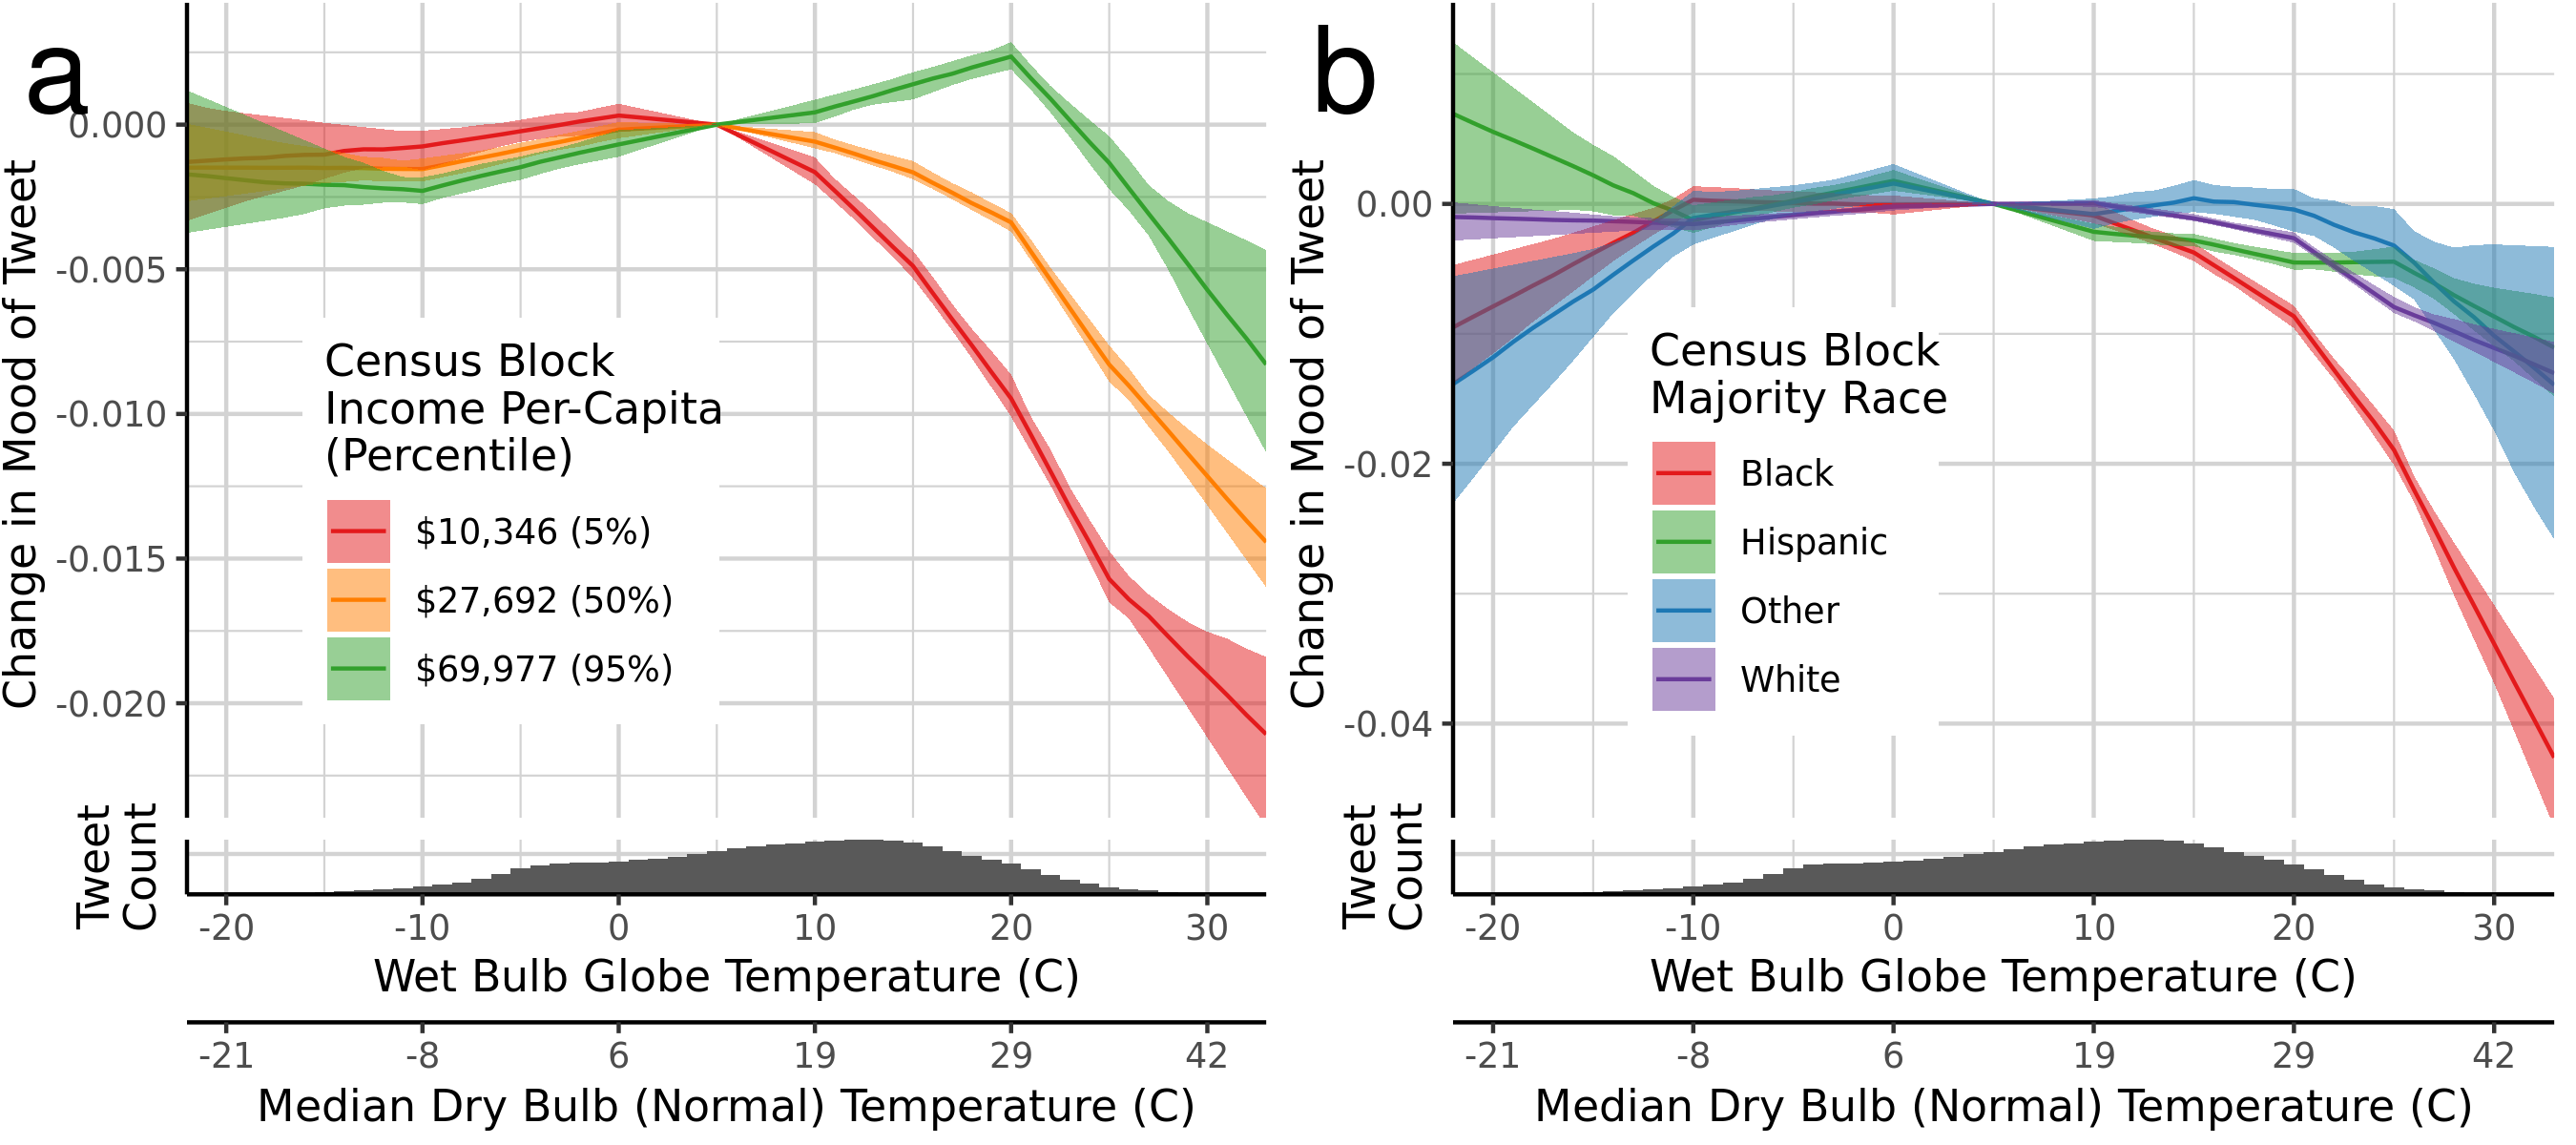
\includegraphics[width=\linewidth]{../res/wbgt_combined.png}
 \caption{Effect of changes in WBGT on expressed mood as moderated by neighborhood income (a) and race (b).}
\label{fig:hetero}
\end{figure}

Finally, given that both low-income and majority black neighborhoods are more vulnerable to heat waves, we model the combined effects of race and income together to explore the intersection of these two types of vulnerability. Specifically, we model how the relationship between temperature and mood is moderated by the interaction between a neighborhood's per-capita income and the percentage of a neighborhood's inhabitants that are black. Additionally, we compare AICs for models with no term for vulnerability, a race term for vulnerability, an income term for vulnerability, and both race and income terms for vulnerability.

\begin{minipage}{.65\textwidth}
\centering
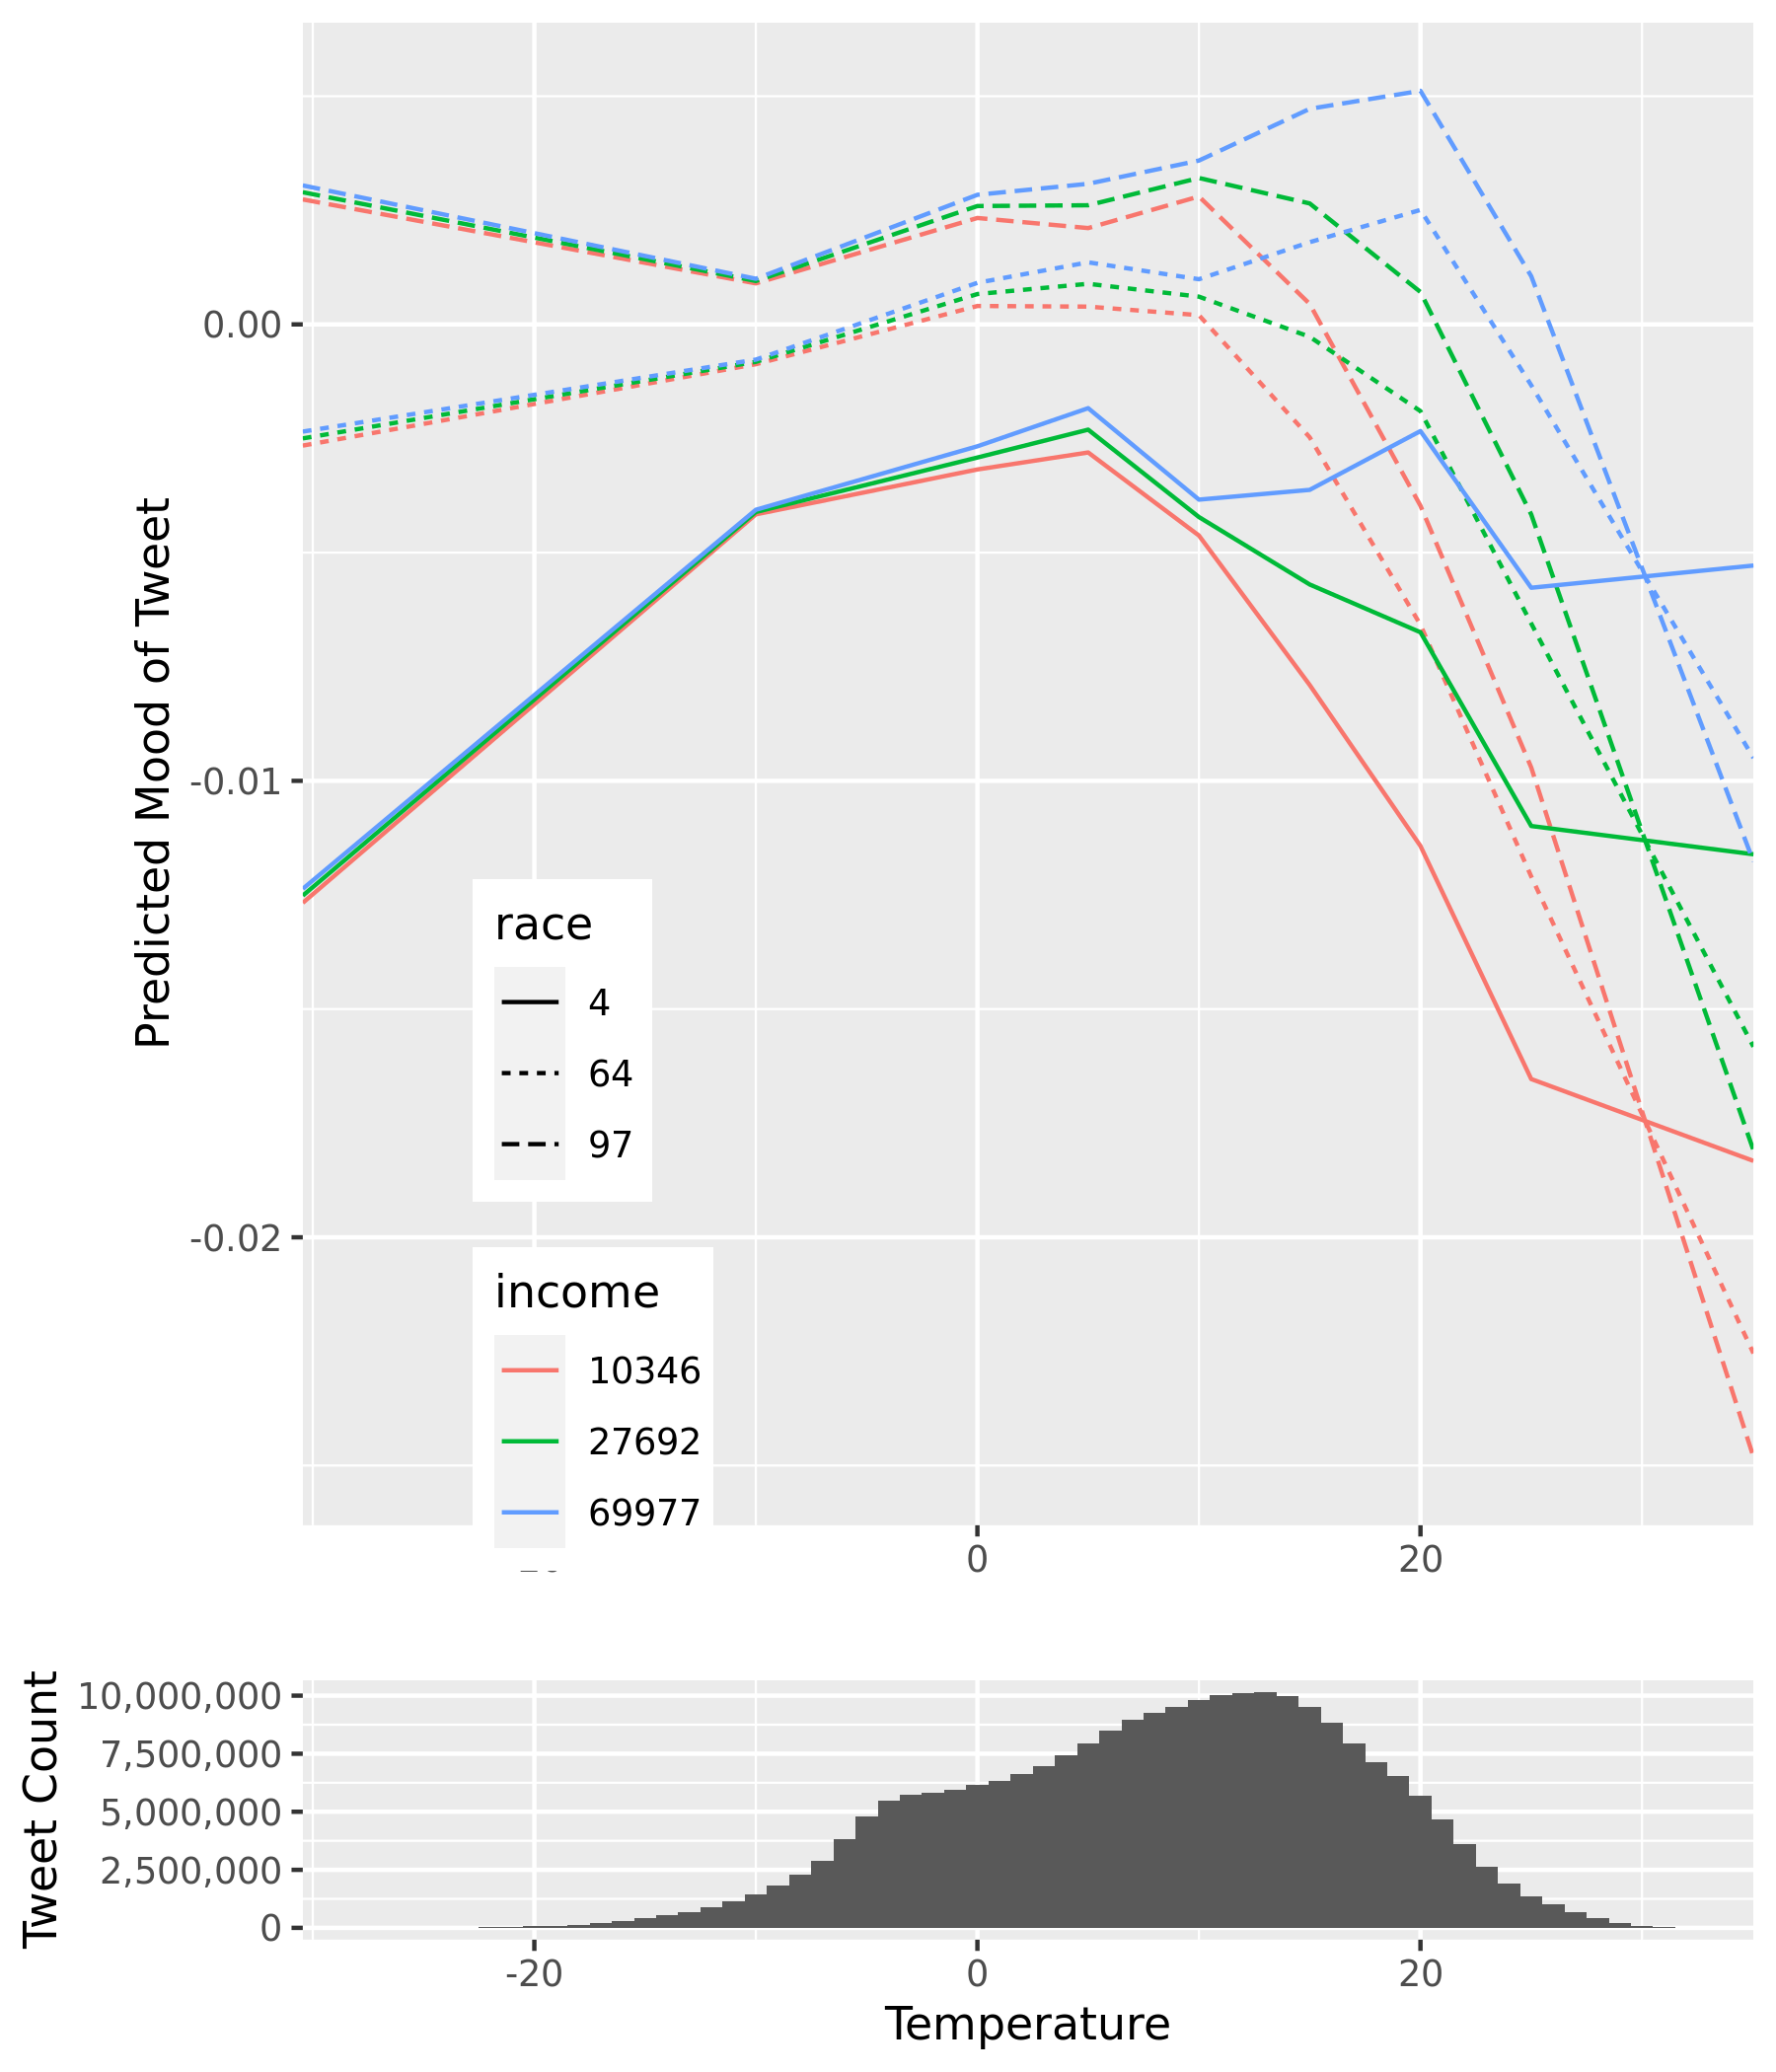
\includegraphics[width=\textwidth]{../res/wbgt-income-race.png}
\captionof{figure}{Relationship between WBGT and mood from text in tweets, moderated by the interaction of race and income.}
\label{fig:race-income}
\end{minipage}\hfill
\begin{minipage}{.35\textwidth}
\centering
\begin{tabular}{| l | l |}
\hline
Terms & AIC \\
\hline
Neither & 277270561 \\
Income & 277182239 \\
Race & 277143579 \\
Both & 277108676 \\
\hline
\end{tabular}
\captionof{table}{Akaike information criterion (AIC) of models with interaction terms for race, income, both race and income, as well as neither race nor income. The model with the best fit by AIC includes both race and income interaction terms.}
\label{tab:aics}
\end{minipage}

Graphing the combined effects of race and income, we find that race has a larger impact on vulnerability than income (see Fig. \ref{fig:race-income}). A fully black neighborhood at any income level will be much more impacted by heat than a poor neighborhood with few black inhabitants. Additionally, neighborhoods that are largely black are also more affected by cold temperatures, although there is no clear effect of income moderating the relationship between cold temperatures and mood. Using AIC as an indicator of how different terms affect model quality (see Tab. \ref{tab:aics}), we find that a model including both terms performs the best, indicating that both race and income matter for the impact of heat on mood. However, including only a race term improves the model more than including only an income term, further supporting the conclusion that race is more important than income for explaining the vulnerability of mood to heat.

\subsection*{Comparison With Other Events}
We compared the expressed mood from exposure to temperatures to two other events associated with impacts on mood and other mental health outcomes: the weekly change from Saturday to Monday, as well as the impact of a major natural disaster (see Fig. \ref{fig:compare}). For this comparison, we define heat impact as the changes in mood associated with temperatures increasing from 5\textdegree C WBGT (12\textdegree C/54\textdegree F) to 25\textdegree C WBGT (36\textdegree C/97\textdegree F); we define weekly changes as the difference between the mean Saturday mood and the mean Monday mood, calculated across the entire data set; and we define the impact of Hurricane Sandy as the change in mood from the week before the hurricane made landfall to the week after, calculated for only impacted counties. Both of these events are associated with mental health impacts: the decrease in expressed mood on Twitter from Saturdays to Mondays mirrors mirrors the weekly dynamics of suicide rates \cite{CDC2021}, while Hurricane Sandy was associated with mental health effects on victims including increased anxiety, PTSD, and depression \cite{Schwartz2017Aug, Lieberman-Cribbin2017}.

\begin{figure}[H]
 \centering
 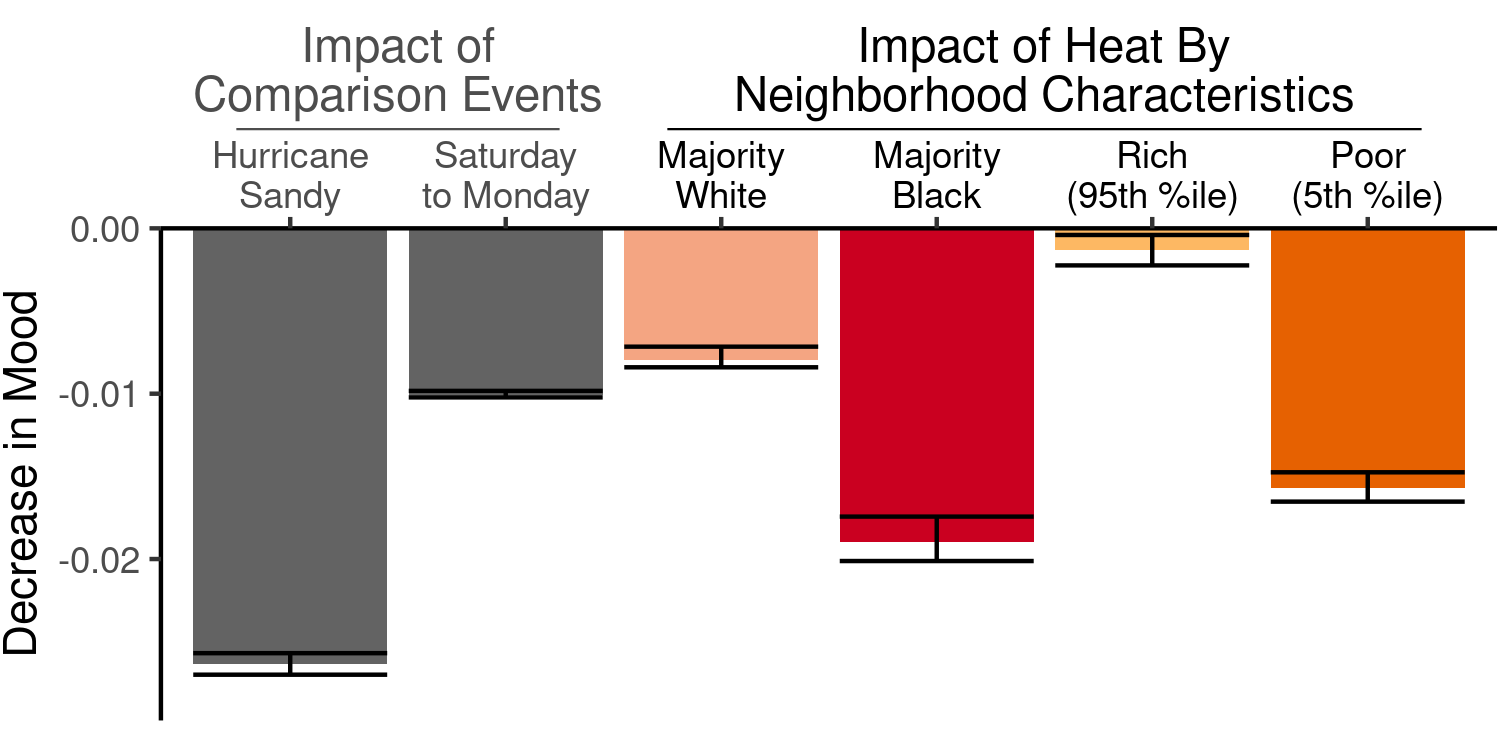
\includegraphics[width=0.66\linewidth]{../res/comparison_plot.png}
 \caption{Decline in mood as temperature changes from mild to high across different neighborhood types, compared with the impacts of the change from Saturday to Monday, as well as the change associated with Hurricane Sandy.}
 \label{fig:compare}
\end{figure}

We find that the decline in mood in wealthier and majority white neighborhoods from exposure to increasing temperatures is less than the average weekly change in mood from Saturday to Monday (see Fig. \ref{fig:compare}). Conversely, the effects of exposure to increasing temperatures in poorer and majority Black neighborhoods are much larger than the average weekly change in mood. Additionally, the impacts of exposure to these changes in temperature for the more vulnerable neighborhoods are close in severity to the impact on mood from experiencing a major hurricane.

\subsection*{Temperature Effects by Time of Day}
In addition to providing data with high spatial resolution, Twitter data also comes with very high temporal resolution as each tweet is time-stamped. Thus, we were able to examine the impact of heat on mood over the course of the day (Fig. \ref{fig:ts-wbgt}). We found that heat is associated with improved mood for a brief period in the late morning, and then has a negative effect on mood during the latter half of the day, with a consistent effect from noon until 9pm. This effect weakens in the early evening through midnight, and then increases substantially throughout the night. Heat has the greatest effect on expressed mood at 6am, an effect over twice as large as during the day.

\begin{figure}[H]
 \centering
 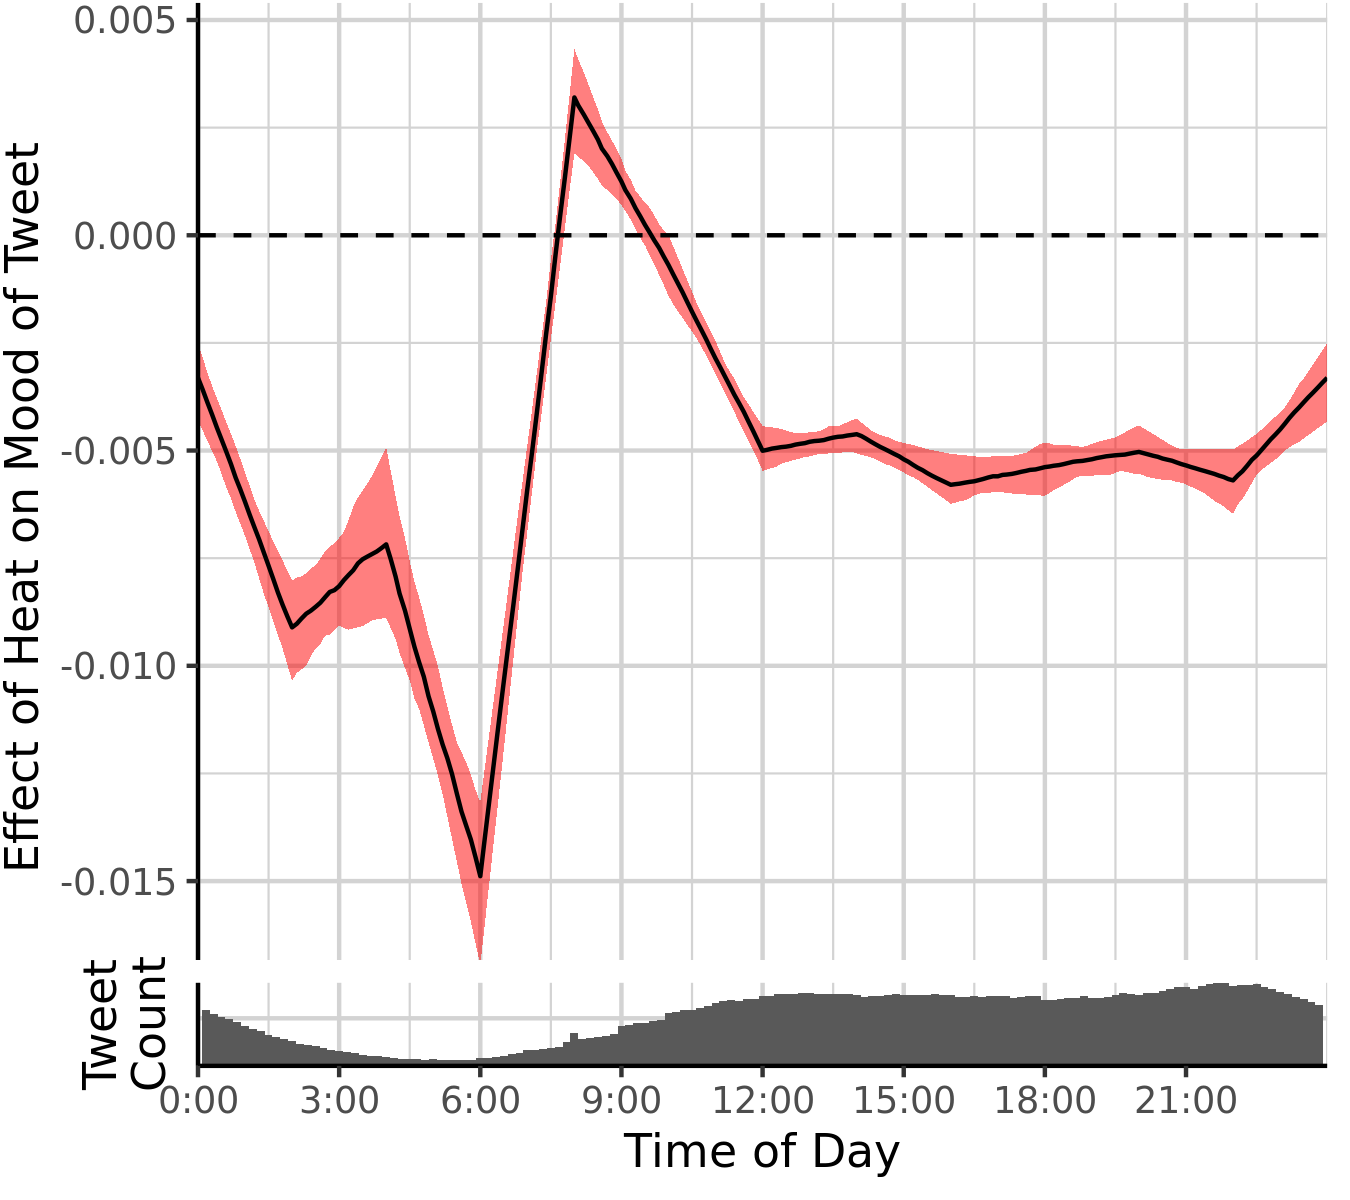
\includegraphics[width=0.5\linewidth]{../res/ts_heat.png}
 \caption{Effects of rising temperatures on mood by hour of the day, with a 95\% confidence interval. The value shown is the predicted change in VADER score for a 10\textdegree C WBGT increase in temperatures.}
 \label{fig:ts-wbgt}
\end{figure}

\section*{Discussion}
% Benefits of Twitter data/overview of findings
We find that Twitter data offers significant advantages for observing environmental effects on human well-being due to its very fine spatio-temporal resolution. We were able to pair each tweet with the local temperature at the time of the tweet, and found a clear association between increasing temperatures and declining mood. Moreover, we were able to show heterogeneity in vulnerability by neighborhood characteristics, improving on previous findings that found no heterogeneity at the county level \cite{Burke2018Aug, Mullins2019Dec}.

% Compare weekly changes in mood to weekly changes in suicides
We found that the change from optimum temperature of 5\textdegree C WBGT (12\textdegree C/54\textdegree F) to a higher temperature of 25\textdegree C WBGT (36\textdegree C/97\textdegree F) is associated with an overall decrease in mood of 0.01. This is similar to the degree of change in mood over the course of a week from a Monday nadir (0.1268) to a Saturday peak (0.1372), a weekly change associated with an increase in suicides of 23\% over the course of the study period \cite{CDC2021}. Thus, while research on linkages between expressed mood and other mental health outcomes like suicides and hospitalizations is still nascent, there are clear similarities in patters of mood and suicides at some time scales. Moreover, like mood, suicides are affected by higher temperatures. While the mood expressed on Twitter is only a proxy for mental health and not a direct measurement, the two phenomena have similar temporal patterns and respond similarly to heat. Thus, the changes in expressed mood we observe at neighborhood scales are very likely indicative of mental health outcomes such as suicides and hospitalizations.

% Discuss the NOVELTY: quote Burke and Mullins, refute their interpretations, people have said XX, but we have shown ~XX.
% Variations in vulnerability also indicates ADAPTATION
Previous work conducted with county-scale data found no heterogeneity in mental health vulnerability by income. Such analyses have led to conclusions that the mental health effects of climate change will be uniform, least in developed countries, and that adaptation with technologies like air-conditioning will not mitigate the mental health effects of climate change. For example, Mullins et al. conclude that ``individuals have not been able to successfully reduce the negative effects of higher temperatures on mental health" \cite{Mullins2019Dec}. Contrary to these analyses, we found large heterogeneity in vulnerability by neighborhood racial composition and per-capita income. This suggests that the mental health effects of climate change will not be uniform and, like other impacts, will fall disproportionately on the poor and vulnerable. More positively, it does suggest that adaptation is possible, and, for communities with infrastructure and working conditions similar to those of higher-income Americans, the effects of high temperatures on mental health may be addressable. Additionally, our results suggest that reducing existing discrimination in housing and employment would contribute narrowing racial gaps in vulnerability and be an important:w
adaptation strategy.

Counter to previous studies, we find that the highest temperatures disproportionately affect poor and marginalized populations. Moreover, we find that majority Black neighborhoods are much more affected by higher temperatures than neighborhoods with a non-Black majority. This is surprising, given that Hispanic peoples can be marginalized in income, language and housing. This may be because the ethnic category of Hispanic is more broad and encompasses many more groups with more diverse histories and living conditions than Black Americans. It may also be due to that fact that more marginalized and heat-vulnerable Hispanic people were more likely to tweet in the Spanish language, which we did not include our analysis. Additionally, there are many other marginalized groups in America, particularly indigenous people, that we did not have sufficient data to examine with respect to heat and mental health. Finally, while race is correlated with income in the US, we find that neighborhood racial characteristics more directly contributed to vulnerability to heat, independent of income. This suggests that racism and patterns of housing discrimination like the legacy of redlining contribute to making Black Americans more vulnerable to heat, even at similar levels of income as other groups. Thus, our study shows that the degree of vulnerability to heat stress is less related to a single category or variable (e.g., race or income) but is more likely related to a variety of complex, intersecting dimensions like combinations of race and housing \cite{Kuran2020Nov}. 

% Connect to bigger literature on vulnerability
This study shows the importance of examining heterogeneities in vulnerability in analyses of climate change impacts, as well as the importance of measuring impacts at fine spatial scales. Within in relatively wealthy nation of the United States, we find large heterogeneity in vulnerability. This adds to the growing literature showing that the impacts of climate change will be highly unequal and disproportionately borne by the poor and marginalized \cite{Thomas2019Mar}. Moreover, given that more impoverished neighborhoods in the United States see greater mental health impacts during heatwaves, it is likely that heat waves have a much greater mental health impact throughout the developing world, where temperatures are expected to be much higher \cite{Raymond2020May}, heatwaves are already under-counted \cite{Harrington2020Sep}, and adaptive technologies like air conditioning are more scarce \cite{Biardeau2020Jan}.

In addition to exploring heterogeneities in vulnerability, using twitter data lets us explore how the effect of heat varies by time of date and infer possible important pathways in the heat-mental health relationship. Recent research has suggested that the impacts of heat on sleep quality may play a large role in the observed mental health effects of heat \cite{Obradovich2017May, Mullins2019Dec}, and our temporal analysis largely supports this hypothesis.  We found much stronger effects of heat on expressed sentiment in the early morning, adding weight to the sleep quality pathway linking heat and mental health that other authors have found.  This suggests that efforts to improve mental health during heat waves may have the largest impact by focusing on providing electricity and air conditioning at night.


% Caveats
% Mood is a fuzzy indicator but we have BIG DATA
While these findings are robust to different model specifications and metrics of mood, a limitation of data from Twitter is that a tweet is not a precise measurement of a discrete mental health outcome and only provides a rough indicator a user's mental state based on the vocabulary in the tweet. Moreover, while mood/sentiment analysis algorithms have gotten increasingly sophisticated at estimating the mood in a body of text, a user's expressed mood in a tweet is highly variable and is mostly affected by factors like current events and the user's personal life, with local weather conditions having only a small impact. We overcome this limitation by using an extremely large data set of 243 million tweets, allowing us to control for a wide variety of spatial and temporal effects to estimate population-level changes in mood in relation to the weather.

One caveat associated with this data is that we were only able to locate the tweets within the census block where the tweet was sent - we did not to infer where the person sending the tweets typically lived or where they had been. Many low-income and Black people commute during the day to work in the service sector in higher-income areas, so these results may in fact under-estimate the impacts of higher temperatures on mental health for poor and minority individuals. Moreover, in some cases the income level of a census block may be only weakly indicative of the wealth of the people who are typically found that census block. For example, some public spaces are estimated to have very low income levels even though people from a variety of income levels may occupy those spaces throughout the day. Additionally, neighborhoods of young college students are also typically estimated to have low income levels, even through college students are wealthier than the average American. Again, these issues mean we are likely under-estimating the true effect of heat on mental health for poor and Black people. A final issue with using Twitter data is that, while Twitter is used by more than one in five Americans, Twitter users may not be representative of the general population, as they are typically younger, wealthier, and more educated \cite{Pew2020Sep}. Nevertheless, we found a large volume of tweets across all neighborhood types.

% NCC doesnt have a "conclusion" section, but this is intended as an overall summary paragraph
While climate change will have widespread and severe impacts on human well-being, our work emphasizes just how highly unevenly these impacts will be distributed. People with more money, access to aid and infrastructure, and who belong to ethnic groups in power are less affected by climate shocks and natural disasters and more able to adapt \cite{bullard2012wrong}. While the physical health impacts of these shocks are more visible and easy to measure, the mental health impacts of climate change are also causing severe human suffering and there is no reason to believe they will not also be highly unevenly distributed. Thus, there are strong theoretical priors behind the hypothesis that low-income and marginalized people are more vulnerable to the mental health impacts of higher temperatures, even though previous work at coarse spatial scales had not found such an effect. By using fine-scale Twitter data, we show that there are indeed stark differences in the mental health impacts of heat among neighborhoods in the United States. These findings have significant implications for urban planning, climate and environmental justice, and mental health.

\section*{Methods}
\subsection*{Tweets \& Mood}
We used data from 243 million geo-located English-language tweets from the continental United States from the years 2009 to 2019. The Twitter data consists of publicly posted messages, or tweets, that are short status messages users post to the platform. We only considered users’ original content, thus did not include retweets in our analysis. Additionally, we excluded all tweets that contained weather-related terms, to ensure that the mood expressed in the tweets was reflective of a user's mental state, and not a commentary on the weather.

Expressed mood is a widely used metric to assess mental health and well-being from posts on social media platforms. We use the VADER metric to assess the mood of Twitter posts as it was specifically designed for microblogs like Twitter \cite{hutto2014vader}. The VADER (Valence Aware Dictionary for Sentiment Reasoning) corpus \cite{gilbert_vader_2014} is a lexical, rule-based sentiment analysis tool that is specifically attuned to moods expressed on social media and includes several features, as:

\begin{itemize}
 \item Incorporating lexical features common to informal media, such as slang (``sux"), and acronyms (``lol").
 \item Negations (``\textit{not} good", ``\textit{wasn't} bad")
 \item Punctuation (``Good!!!")
 \item Word shape, such as capitalization (``The movie was AMAZING")
 \item Emoticons and emojis (``:-)", ``\emojismile")
 \item Degree modifiers (``very excellent" or ``kind of crappy")
\end{itemize} 

The VADER method yields a value for the mood of a tweet, with a score of 0 for neutral tweets, a score $> 0$ for positive-mood tweets and a score $< 0$ for negative-mood tweets. While we ultimately settled on using VADER for assigning sentiment scores, we also conducted analyses using the Hedonometer and AFINN mood analysis methods, with similar results (See Supplement).

\subsection*{Weather}
We used data on local weather conditions from the North American Land Data Assimilation System (NLDAS), a gridded product developed by several collaborative institutions, including NOAA, NASA, Princeton University, and the University of Washington. This dataset is available at an hourly temporal resolution, and at 1/8th decimal degree spatial resolution, and integrates a large quantity of observation-based and modeled data \cite{xia_continental-scale_2012}. We extracted temperature, specific humidity, air pressure, total precipitation, shortwave radiation, and wind speed for the exact hour and location of each tweet. 

We calculated the Wet Bulb Globe Temperature (WBGT) at the time and location of each tweet as temperature metrics that account humidity and other factors can better account for the impacts of heat stress on human health and well-being. The WBGT is the temperature that a wet globe thermometer would read in direct sunlight, and gives a reading lower than a dry bulb temperature due to evaporative cooling. The WBGT can be estimated given normal temperature, relative humidity, solar radiation, and wind speed. Because evaporative cooling is how humans cool themselves through perspiration, this temperature better indicates the heat stress that people are experiencing \cite{budd2008wet}. Metrics like WBGT that account for the effects of humidity and other factors on heat stress have been associated with diminished economic output \cite{rao2020projections}, increased crime \cite{hu2017impact}, increased mortality \cite{chien2016spatiotemporal, armstrong2019role}, and worsened mental health outcomes \cite{vida2012relationship, ding2016importance}.

We derived relative humidity using methods described by Bolton et al. \cite{bolton_computation_1980} which use temperature, specific humidity, and pressure. We then calculated the WBGT using the formula described by Heo et al. \cite{heo2019comparison}.

Throughout the paper we give the median dry bulb temperature observed at each given wet bulb temp degree across our data set. It should be noted, however, that a wide range of dry bulb temperatures can be associated with a given wet bulb globe temperature, depending on humidity, wind speed, and sunlight.

\subsection*{Socio-Economic Data}
We used data from the American Community Survey (ACS) administered by the US Census to estimate income levels and the racial composition of neighborhoods where tweets were located. Data was at the level of the census block group, the smallest unit for which the US Census releases public data. Following Census categories, we report racial characteristics of neighborhoods as majority population of four broad racial categories - non-Hispanic Black, non-Hispanic white, Hispanic of any race, and other, which includes Native American, multi-racial, Asian-American and Pacific Islander. 

The ACS data covers five-year periods. We therefore matched each tweet with census block group data from the year at the middle year of each survey's five-year range. For example, tweets from 2014 were matched to data from the 2012-2016 ACS. Because the most recent available ACS was from 2014-2018, all tweets from year years greater than 2016 were matched to this dataset. We used data from the Integrated Public Use Microdata Series (IPUMS USA) National Historical Geographic Information System (NHGIS) service provided by the University of Minnesota \cite{ruggles2018ipums}.

We use the mean annual income per capita from the ACS, standardized so that values for each year are in 2019 dollars. For racial categories, we combined the various categories provided by the ACS into four racial groups: non-Hispanic white, non-Hispanic Black, Hispanic of any race, and an "other" category for non-Hispanic people who were neither Black nor white, such as Asian, Native American, or mixed-race people.

We present income and racial percentiles based on the observed percentiles across all tweets in our data set.
 
\subsection*{Modeling}
We assessed how expressed mood is affected by Wet Bulb Globe Temperature using segmented regressions, controlling for precipitation, shortwave solar radiation (sunshine), as well as the following spatio-temporal fixed effects: day of the week, time of day, day of the year, year, month, and county. 

Our initial model (for Fig. \ref{fig:wbgt}) takes the following form:

\begin{equation}
 y = \beta_0 + f_t(t) + \beta_p p + \beta_s s + \Phi + \epsilon
 \label{mod:1}
\end{equation}

Where $y$ is the mood of a tweet, $t$ is the wet bulb globe temperature at the hour of the tweet, $p$ is a binary variable indicating whether it rained at the hour of the tweet, $s$ is the income shortwave radiation, or sunshine, in $W/m^2$, at the hour of the tweet, $\Phi$ is the spatio-temporal fixed effects, $\epsilon$ is the normally-distributed errors, and $f_t$ represents the segmented effect for $t$, with knots at -10\textdegree, 0\textdegree, 5\textdegree, 10\textdegree, 15\textdegree, 20\textdegree, and 25\textdegree C WBGT. We estimate the 95\% confidence interval of all our models using 80-fold bootstrapping. 

To examine how income and racial groups moderate the effect of heat on mood, we extend our model to the following form:

\begin{equation}
 y = \beta_0 + f_t(t) + f_{mt}(m t) + \beta_p p + \beta_{mp} m p + \beta_s s + \beta_{ms} m s + \Phi + \epsilon
 \label{mod:2}
\end{equation}

Where $m$ is either the log-transformed average income in the census block where the tweet originated, or a dummy variable for the four racial categories. We specify alternative models where income is a dummy variable in three bins and were race is a continuous variable for the percent of a census block population that is white These alternative specifications yield similar results. We also examine the effects of rainfall and sunshine on mood by income and race. These alternative specifications and analysis of rainfall and sunshine effects are available in the Supplement.

In addition to our models exploring how income and race moderate the effect of heat on mood individually, we fit an additional model with an interaction terms for both race and income. Due to the complexity of a model with segmented terms interacting with two different variables, using a categorical variable for race would have yielded a model matrix too large for the largest cloud virtual machine available to us. Thus, we used a continuous metric for both income as well as race (percent black). This model extends our main model to the following form:

\begin{equation}
 y = \begin{tabular}{l}
 $\beta_0 + f_t(t) + f_{m_{i}t}(m_{i} t) + f_{m_{r}t}(m_{r} t) + 
 \beta_p p + \beta_{m_{r} p} m_{r} p + 
 \beta_{m_{i} p} m_{i} p + \beta_{m_{i} m_{r} p} m_{i} m_{r} p + $
 \\
 $\beta_s s + \beta_{m_{i} s} m_{i} s + 
 \beta_{m_{r} s} m_{r} s + \beta_{m_{i} m_{r} s} m_{i} m_{r} s + 
 \Phi + \epsilon$
 \end{tabular}
 \label{mod:race-inc}
\end{equation}

In this new model, $m_{i}$ is average income in the census block where the tweet originated, while $m_{r}$ is the racial composition of the census block.

Finally, we fit a model for how heat affects mood by time of day. For this analysis, we used a varying-coefficient model, where the effect of heat is linear, but the coefficient for the effect varies non-linearly as a function of the time of day. Because we modeled the effect of heat as linear, we excluded all tweets with an observed temperatures less than 5\textdegree C WBGT so that we were only including values at which our previous analyses suggested the heat-mood relationship is monotonic. This final model took the following form:

\begin{equation}
 y = \beta_0 + f_h(h)t + \beta_p p + \beta_s s + \Phi + \epsilon
 \label{mod:tod}
\end{equation}

In this final model, $f_{h}$ is the coefficient for temperature, $t$, and varies non-linearly by time of day, $h$. To ensure that the effect $f_{h}$ is cyclical, we estimated $f_{h}$ using 2nd-order B-splines, also known as a tent function basis \cite[Chapter~4.2]{wood2017generalized}, with knots every two hours.

\section*{Acknowledgements}
%Official SESYNC wording
This work was supported by the National Socio-Environmental Synthesis Center (SESYNC) under funding received from the National Science Foundation DBI-1639145. Additionally, computational resources for this project were provided for the Microsoft Azure cloud through Microsoft's AI for Earth program.

This data came from Twitter via the University of Vermont’s (UVM) agreement with Twitter to access its streaming API - colloquially referred to as the Decahose. The UVM special agreement with Twitter allows for access to this data for research and analysis purposes and this work complies with all the terms of service for Twitter and UVM. 

%\printbibliography
\bibliography{TextDataClimateShocks}

\section*{Author Contributions}
Author contributions: M.C., J.O.-G., A.S. and P.B. designed the research and modeling strategy; A.S. provided data; M.C and Z.L. prepared data; M.C. and J.O.-G. analyzed data; and M.C., J.O.-G., P.A.W., and J.L. wrote the paper.

\noindent This paper was the result of a SESYNC graduate pursuits project co-lead by M.C. and J.O.-G.

\end{document}
